\mySection{7.3 Deriving the Distribution of $\frac{\overline{Y}-\mu}{S/\sqrt{n}}$}
%-------------- start slide -------------------------------%{{{ 7.21
\begin{frame}
	% {\S\: 7.3 Deriving the Distribution of $\frac{\overline{Y}-\mu}{S/\sqrt{n}}$}
\begin{enumerate}
	\item[Def.] \textcolor{yellow!80!black}{\bf Sampling distributions}\\[1em]
		Distributions of \underline{\it functions of random sample} of given size.  \\
		\hspace{8.5em}  statistics / estimators
		\vfill
	\item[E.g.] A random sample of size $n$ from $N(\mu,\sigma^2)$ with $\sigma^2$ known.\\[1em]
		Sample mean $\overline{Y} = \frac{1}{n}\sum_{i=1}^n Y_i\sim N(\mu,\sigma^2/n)$
		\vfill
	\item[Aim:] Determine distributions for \\[2em]
		\begin{center}
			\begin{tabular}{c|c}
				Sample variance $S^2:=\frac{1}{n-1}\sum_{i=1}^n\left(Y_i-\overline{Y}\right)^2$ & {\it Chi square distr.}\\[1em]
				$\displaystyle T:=\frac{\overline{Y}-\mu}{S/\sqrt{n}}$ & {\it Student t distr.}\\[1em]
				$\displaystyle \frac{S_1^2}{\sigma_1^2}\bigg/\frac{S_2^2}{\sigma_2^2}$ & {\it F distr.}
			\end{tabular}
		\end{center}
\end{enumerate}
\end{frame}
%-------------- end slide -------------------------------%}}}
%-------------- start slide -------------------------------%{{{ 7.22
\begin{frame}
\begin{enumerate}
	\item[Thm \small 7.3.1.] Let $U=\sum_{i=1}^m Z_j^2$, where $Z_j$ are independent
		$N(0,1)$ normal r.v.s. Then
		\[
			\text{$U\sim$ Gamma(shape=$m/2$, rate=$1/2$).}
		\]
		namely,
		\[
			f_U(u) =  \frac{1}{2^{m/2}\Gamma(m/2)}u^{ \frac{m}{2}-1}e^{-u/2}, \qquad u\ge 0.
		\]
		\vfill
	\item[Def \small 7.3.1.] $U$ in Thm 7.3.1 is called \textcolor{yellow!80!black}{\bf chi square distribution} with $m$ dgs of freedom.
\end{enumerate}
\end{frame}
%-------------- end slide -------------------------------%}}}
%-------------- start slide -------------------------------%{{{ 7.23
\begin{frame}[fragile]
	\begin{enumerate}
		\item[Proof.] We first consider the case when $m=1$. In this case,
			\begin{align*}
				F_{Z^2}(u) & = \bbP\left(Z^2\le u\right)                     \\
                   & = \bbP\left( -\sqrt{u}\le Z \le \sqrt{u}\right) \\
                   & = 2 \bbP(0\le Z\le \sqrt{u})                    \\
                   & = \frac{2}{\sqrt{2\pi}} \int_0^{2\pi} e^{-z^2/2} \ud z
			\end{align*}
		\item[] Differentiating both sides of the above eq. in order to obtain the pdf:
			\begin{align*}
				f_{Z^2}(u) & = \frac{\ud}{\ud u} F_{Z^2}(u)                       \\
                   & = \frac{2}{\sqrt{2\pi}} \frac{1}{2\sqrt{u}} e^{-u/2} \\
                   & = \frac{1}{\sqrt{2} \Gamma(1/2)} u^{(1/2)-1} e^{-u/2},
			\end{align*}
		\item[] which is the pdf of a gamma distribution with $r=\lambda=1/2$.
		\item[] Then adding $m$ independent copies of gamma distributions gives anther gamma
			distribution with $r=m/2$ and $\lambda=1/2$ (See Theorem 4.6.4). \myEnd
	\end{enumerate}
\end{frame}
%-------------- end slide -------------------------------%}}}
%-------------- start slide -------------------------------%{{{ 7.24 Chi Square Table with R
\begin{frame}[fragile]{Chi Square Table}
\begin{center}
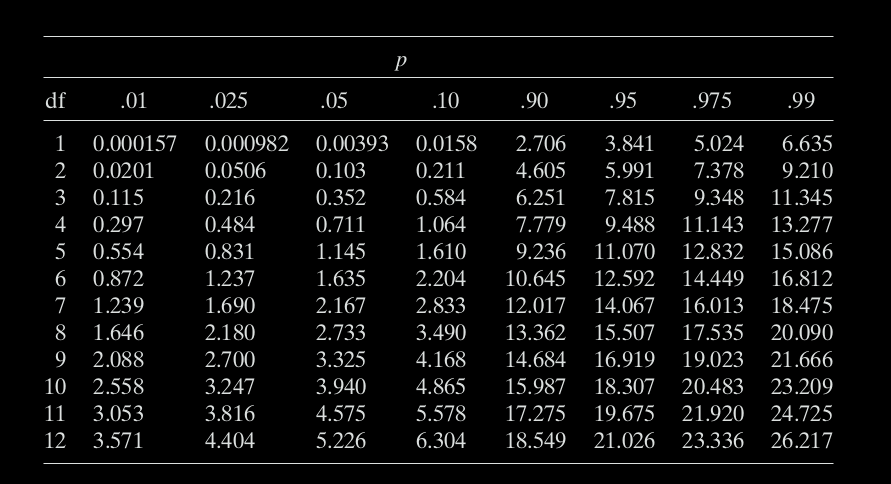
\includegraphics[scale=0.18]{Figure_7-5-2-neg.png}
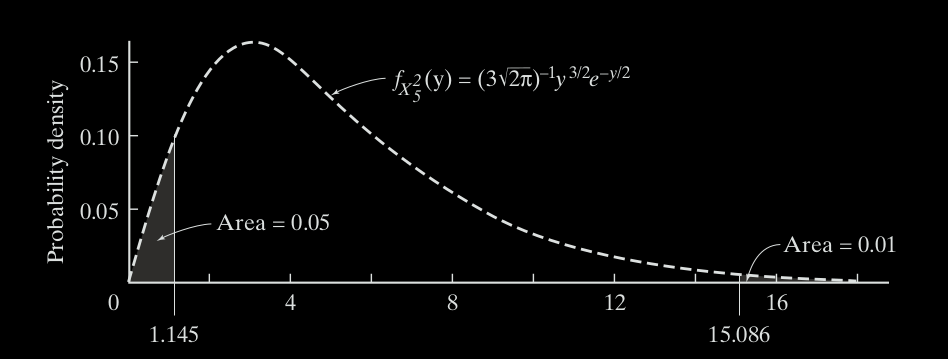
\includegraphics[scale=0.18]{Figure_7-5-1-neg.png}
\begin{align*}
	\bbP(\chi_5^2\le 1.145) = 0.05 & \quad \Longleftrightarrow  \quad \chi_{0.05,5}^2 =1.145 \\
	\bbP(\chi_5^2\le 15.086)=0.99  & \quad \Longleftrightarrow  \quad \chi_{0.99,5}^2 =15.086
\end{align*}
\begin{minipage}{0.3\textwidth}
\begin{lstlisting}
> pchisq(1.145, df = 5)
[1] 0.04995622
> pchisq(15.086, df = 5)
[1] 0.9899989
\end{lstlisting}
\end{minipage}
\qquad\qquad
\begin{minipage}{0.3\textwidth}
\begin{lstlisting}
> qchisq(0.05, df = 5)
[1] 1.145476
> qchisq(0.99, df = 5)
[1] 15.08627
\end{lstlisting}
\end{minipage}
\end{center}
\end{frame}
%-------------- end slide -------------------------------%}}}
%-------------- start slide -------------------------------%{{{ 7.24 Chi Square Table with Python
\begin{frame}[fragile]{Chi Square Table}
\begin{center}
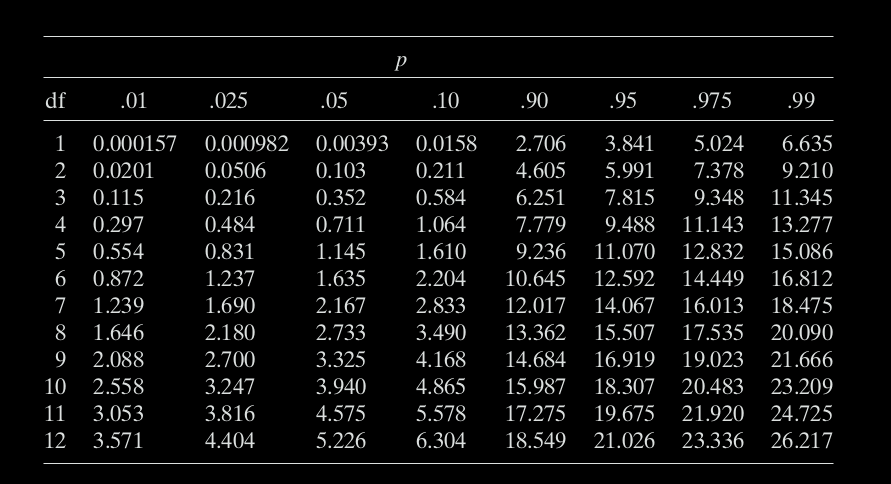
\includegraphics[scale=0.18]{Figure_7-5-2-neg.png}
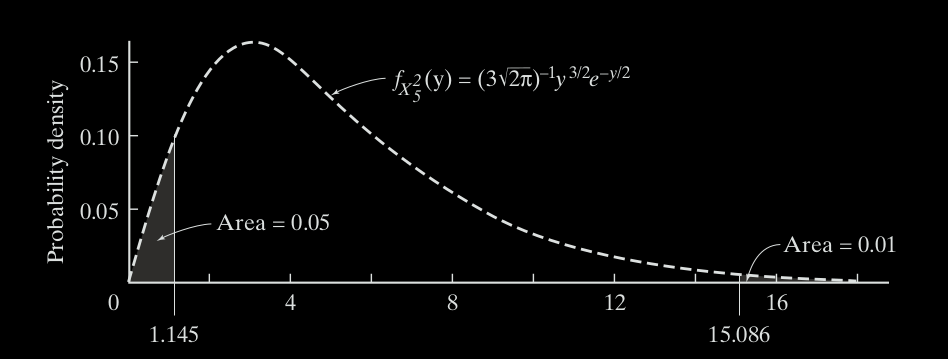
\includegraphics[scale=0.18]{Figure_7-5-1-neg.png}
\begin{align*}
	\bbP(\chi_5^2\le 1.145) = 0.05 & \quad \Longleftrightarrow  \quad \chi_{0.05,5}^2 =1.145 \\
	\bbP(\chi_5^2\le 15.086)=0.99  & \quad \Longleftrightarrow  \quad \chi_{0.99,5}^2 =15.086
\end{align*}
\begin{minipage}{0.4\textwidth}
\begin{lstlisting}[language=Python]
> scipy.stats.chi2.cdf(1.145, 5)
[1]: 0.04995622155207728
> scipy.stats.chi2.cdf(15.086, 5)
[1]: 0.9899988752378142
\end{lstlisting}
\end{minipage}
\begin{minipage}{0.4\textwidth}
\begin{lstlisting}[language=Python]
> scipy.stats.chi2.ppf(0.05, 5)
[1]: 1.1454762260617692
> scipy.stats.chi2.ppf(0.99, 5)
[1]: 15.08627246938899
\end{lstlisting}
\end{minipage}
\end{center}
\end{frame}
%-------------- end slide -------------------------------%}}}
%-------------- start slide -------------------------------%{{{ 7.25
\begin{frame}[fragile]
\begin{enumerate}
\item[Thm \small 7.3.2.] Let $Y_1,\cdots, Y_n$ be a random sample from $N(\mu,\sigma^2)$. Then
\item[] (a) $S^2$ and $\overline{Y}$ are independent.
\item[] (b) $\displaystyle \frac{(n-1)S^2}{\sigma^2} = \frac{1}{\sigma^2}\sum_{i=1}^n\left(Y_i-\overline{Y} \right)^2\quad \sim\quad$ Chi Square($n-1$).
\vfill
\item[Proof.] We will prove the case $n=2$.
	\[
	\overline{Y} =  \frac{Y_1+Y_2}{2},\qquad
Y_1-\overline{Y} =  \frac{Y_1-Y_2}{2}, \qquad
Y_2-\overline{Y} =  \frac{Y_2-Y_1}{2}
	\]
	\[
		S^2 = ...=  \frac{1}{2} \left( Y_1-Y_2 \right )^2
	\]
	\vfill
\item[(a)] It is equivalanet to show $Y_1+Y_2 \perp Y_1-Y_2$. Since they are normal, it suffices to show that
	\[
		\E[(Y_1+Y_2)(Y_1-Y_2)] =
		\E[Y_1+Y_2]
		\E[Y_1-Y_2]
	\]
	\vfill
\item[(b)] $\frac{(n-1)S^2}{\sigma^2} = \left(  \frac{Y_1-Y_2}{\sqrt{2}\sigma} \right)^2 $ and $\frac{Y_1-Y_2}{\sqrt{2}\sigma}\sim N(0,1)$ ...
	\myEnd
\end{enumerate}

\end{frame}
%-------------- end slide -------------------------------%}}}
%-------------- start slide -------------------------------%{{{ 7.26
\begin{frame}
\begin{enumerate}
\item[Def \small 7.3.2.] If $U\sim$ Chi Square$(n)$ and $V\sim$ Chi Square$(m)$, and $U\perp V$, then
\[
F:= \frac{V/m}{U/n}
\]
follows the \textcolor{yellow!80!black}{\bf (Snedecor's) F distribution} with $m$ and $n$ degrees of freedom.
\vfill
\item[Thm \small 7.3.3.] Let $F_{m,n}=\frac{V/m}{U/n}$ be an $F$ r.v. with $m$ and $n$ degrees of freedom. Then
\[
	f_{F_{m,n}}(w) =
	\frac{\Gamma\left(\frac{m+n}{2}\right)m^{m/2}n^{n/2}}{\Gamma(m/2)\Gamma(n/2)} \times
	\frac{w^{m/2-1}}{(n+mw)^{(m+n)/2}}, \quad w\ge 0
\]
\item[] Equivalently,
\[
	f_{F_{m,n}}(w)
	=
	B(m/2,n/2)^{-1} \left(\frac{m}{n} \right)^{\frac{m}{2}} w^{\frac{m}{2}-1}\left( 1+\frac{m}{n}w \right)^{-\frac{m+n}{2}}
\]
\item[] where $B(a,b)=\Gamma(a)\Gamma(b)/\Gamma(a+b)$.
\end{enumerate}
\end{frame}
%-------------- end slide -------------------------------%}}}
%-------------- start slide -------------------------------%{{{ 7.27
\begin{frame}
\begin{enumerate}
	\item[Recall] \phantom{a}\\
	% 	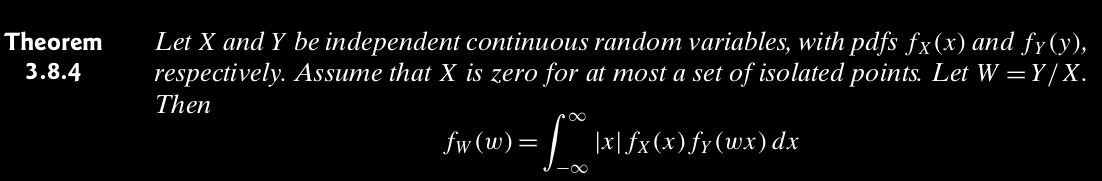
\includegraphics[scale=0.28]{Theorem-3-8-4-neg.png}
	\vfill
	\item[Thm \small 3.8.4] Let $X$ and $Y$ be independent continuous random variables, with
		pdf $f_X(x)$ and $f_Y(y)$, respectively.
	\item[] Assume that $X$ is zero for at most a set of isolated points.
	\item[] Then $W=Y/X$ follows a distribution with pdf:
		\begin{align*}
			f_W(w) = \int_{-\infty}^\infty |x| f_X(x) f_Y(wx) \ud x.
		\end{align*}
		\vfill
	\item[Thm \small 3.8.2] Suppose $X$ is a continuous random variable and $a\ne 0$.
	\item[] Then $Y=aX+b$ follows a distribution with pdf:
		\begin{align*}
			f_Y(y) = \frac{1}{|a|} f_X\left(\frac{y-b}{a}\right).
		\end{align*}
\end{enumerate}
\end{frame}
%-------------- end slide -------------------------------%}}}
%-------------- start slide -------------------------------%{{{ 7.28
\begin{frame}
	\begin{enumerate}
		\item[Proof.] Let us first find the pdf for $W:=V/U$. By Theorem 7.3.1,
			\begin{align*}
					f_V(v) & = \textcolor{yellow}{\frac{1}{2^{m/2}\Gamma(m/2)}v^{(m/2)-1}e^{-v/2}} ,\\
					f_U(u) & = \textcolor{lgtblue}{\frac{1}{2^{n/2}\Gamma(n/2)}u^{(n/2)-1}e^{-u/2}} .
			\end{align*}
		\vfill
		\item[] Then by Theorem 3.8.4, we see that the pdf of $W$ is
			\begin{align*}
				f_W(w) & = \int_{-\infty}^\infty \textcolor{magenta}{|u|} \textcolor{lgtblue}{f_U(u)} \: \textcolor{yellow}{f_V(uw)}\ud u \\
							 & = \int_0^\infty \textcolor{magenta}{u} \textcolor{lgtblue}{\frac{1}{2^{n/2}\Gamma(n/2)}u^{(n/2)-1}e^{-u/2}} \textcolor{yellow}{\frac{1}{2^{m/2}\Gamma(m/2)}(uw)^{(m/2)-1}e^{-uw/2}} \ud u\\
							 & = \frac{1}{2^{(n+m)/2}\Gamma(n/2)\Gamma(m/2)}w^{(m/2)-1}\int_0^\infty u^{\frac{n+m}{2}-1} e^{-\frac{1+w}{2} u}\ud u \\
			\end{align*}
	\end{enumerate}
\end{frame}
%-------------- end slide -------------------------------%}}}
%-------------- start slide -------------------------------%{{{ 7.29
\begin{frame}
	\begin{enumerate}
		\item[] Then by the change of variables, $y=\frac{1+w}{2}u$, we see that
			\begin{align*}
				f_W(w) & = \frac{1}{2^{(n+m)/2}\Gamma(n/2)\Gamma(m/2)}w^{(m/2)-1} \left(\frac{2}{1+w}\right)^{\frac{n+m}{2}} \int_0^\infty y^{\frac{n+m}{2}-1} e^{-y}\ud y \\
							 & = \frac{1}{2^{(n+m)/2}\Gamma(n/2)\Gamma(m/2)}w^{(m/2)-1}  \left(\frac{2}{1+w}\right)^{\frac{n+m}{2}} \Gamma\left(\frac{n+m}{2}\right)
			\end{align*}
			where the last equality is due to the definition of the Gamma function.
		\vfill
	\item[] Finally, by Theorem 3.8.2, we see that $F=\frac{V/m}{U/n} = \frac{n}{m} W$ follows a distribution with pdf
		\begin{align*}
			f_F(y) & = \frac{m}{n} f_W\left(\frac{m}{n} y\right)\\
             & = \textcolor{yellow}{\frac{m}{n}} \frac{1}{2^{(n+m)/2}\Gamma(n/2)\Gamma(m/2)}\left(\textcolor{yellow}{\frac{m}{n}y}\right)^{(m/2)-1} \left(\frac{2}{1+\textcolor{yellow}{\frac{m}{n}y}}\right)^{\frac{n+m}{2}} \Gamma\left(\frac{n+m}{2}\right) \\[1em]
             & = \cdots \qquad y \ge 0.
		\end{align*}
		\myEnd
	\end{enumerate}
\end{frame}
%-------------- end slide -------------------------------%}}}
%-------------- start slide -------------------------------%{{{ 7.30
\begin{frame}[fragile]
\begin{center}
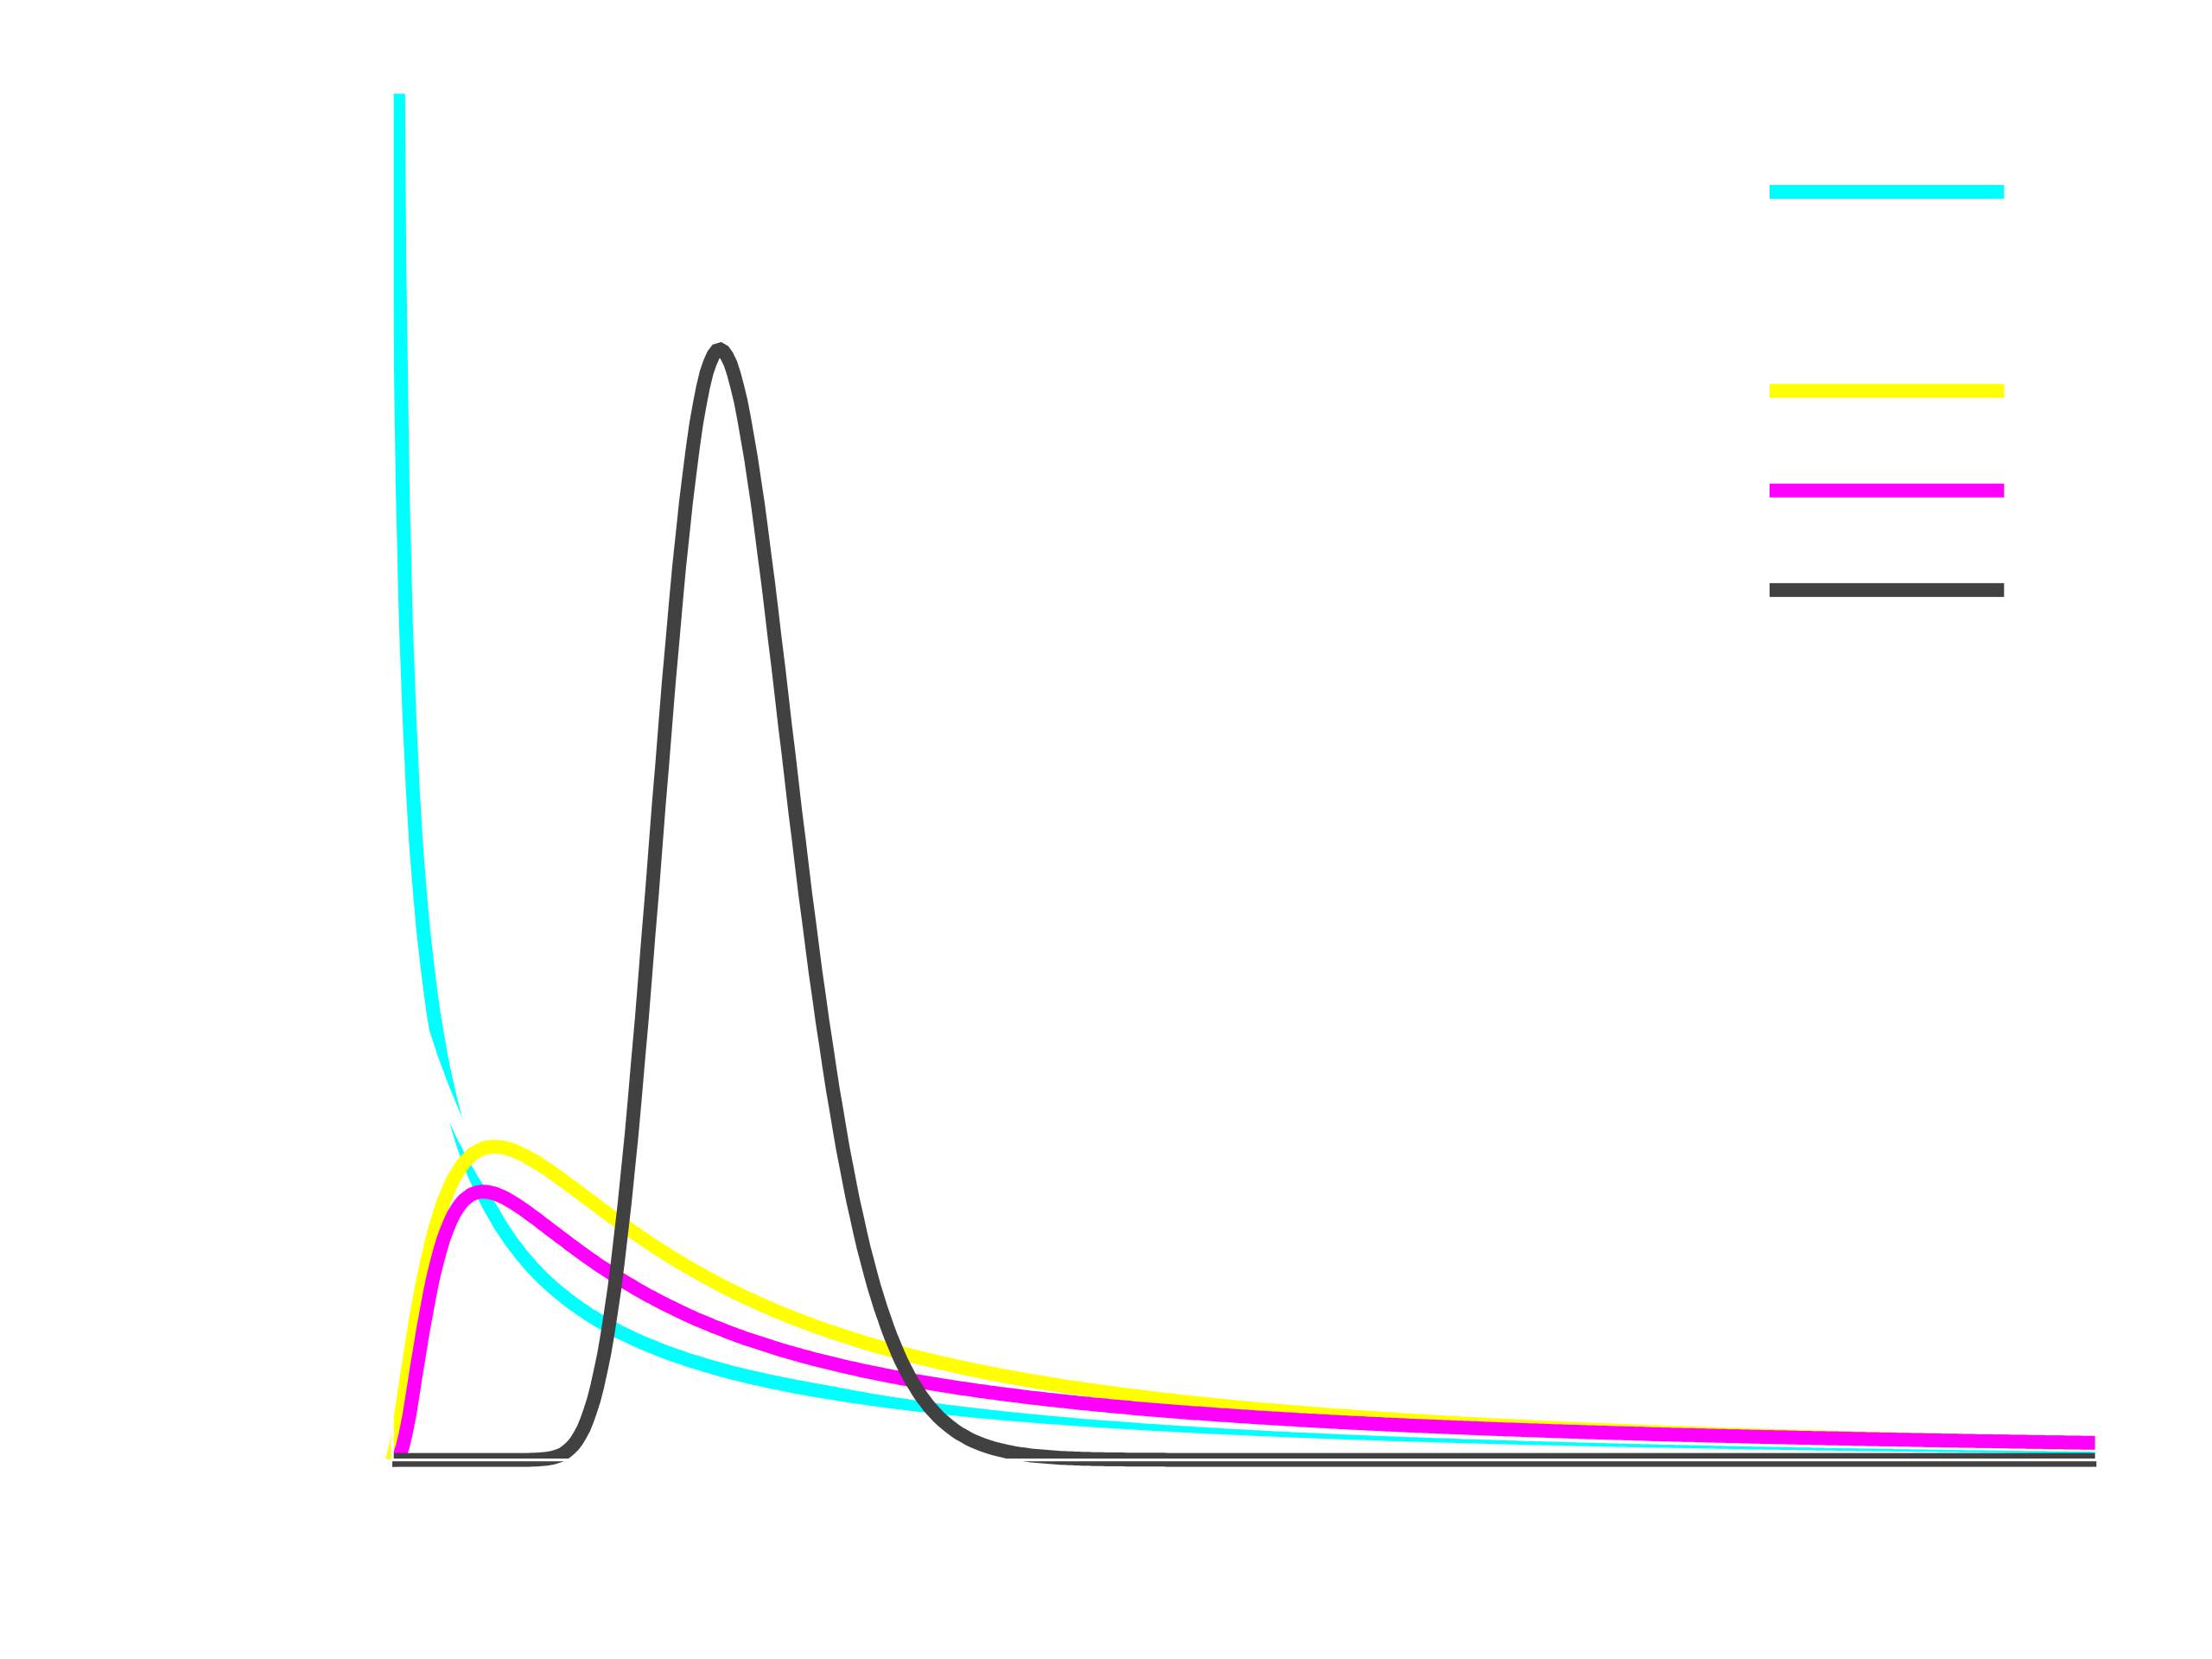
\includegraphics[scale=0.07]{F-distribution_pdf-neg.png}
\end{center}
\vfill
\begin{center}
\begin{minipage}{0.6\textwidth}
\begin{lstlisting}
# Draw F density
x=seq(0,5,0.01)
pdf= cbind(df(x, df1 = 1, df2 = 1),
df(x, df1 = 2, df2 = 1),
df(x, df1 = 5, df2 = 2),
df(x, df1 = 10, df2 = 1),
df(x, df1 = 100, df2 = 100))
matplot(x,pdf, type = "l")
title("F with various dgrs of freedom")
\end{lstlisting}
\end{minipage}
\end{center}
\end{frame}
%-------------- end slide -------------------------------%}}}
%-------------- start slide -------------------------------%{{{ 7.31
\begin{frame}[fragile]{F- Table}
\begin{center}
	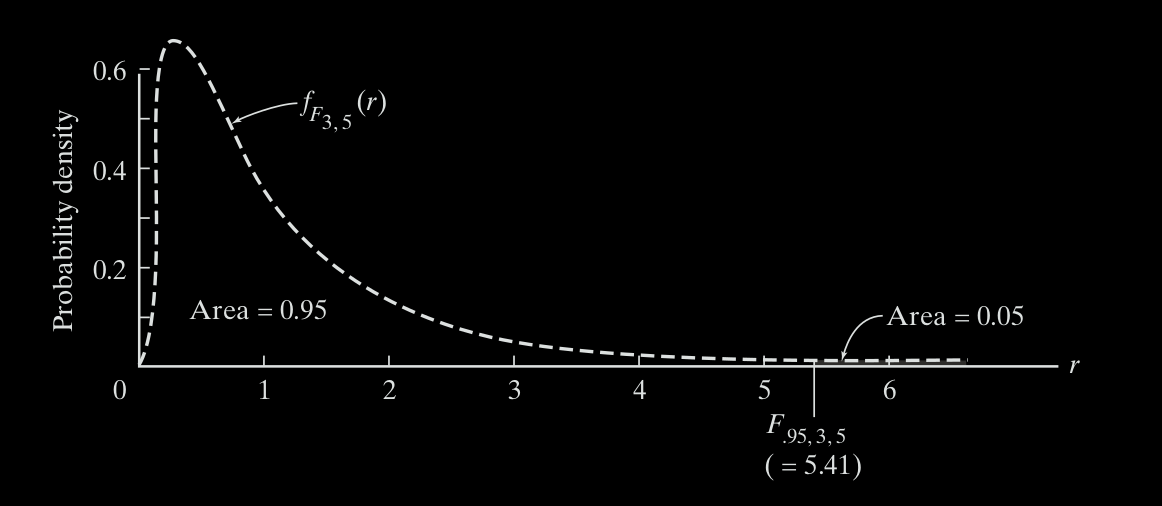
\includegraphics[scale=0.2]{Figure_7-3-1-neg.png}
	\[
		\bbP(F_{3,5}\le 5.41) = 0.95 \quad\Longleftrightarrow\quad
		F_{0.95,3,5} = 5.41
	\]
	\begin{minipage}{0.4\textwidth}
	\begin{lstlisting}
	> pf(5.41, df1 = 3, df2 = 5)
	[1] 0.9500093
	\end{lstlisting}
	\end{minipage}
	\qquad\qquad
	\begin{minipage}{0.4\textwidth}
	\begin{lstlisting}
	> qf(0.95, df1 = 3, df2 = 5)
	[1] 5.409451
	\end{lstlisting}
	\end{minipage}
	\vspace{-1em}

	\begin{minipage}{0.4\textwidth}
	\begin{lstlisting}
	> scipy.stats.f.cdf(5.41, 3, 5)
	[1] 0.9500092950699683
	\end{lstlisting}
	\end{minipage}
	\qquad\qquad
	\begin{minipage}{0.4\textwidth}
	\begin{lstlisting}
	> scipy.stats.f.ppf(0.95, 3, 5)
	[1] 5.40945131805649
	\end{lstlisting}
	\end{minipage}
\end{center}
\end{frame}
%-------------- end slide -------------------------------%}}}
%-------------- start slide -------------------------------%{{{ 7.32
\begin{frame}
\begin{enumerate}
\item[Def \small 7.3.3.] Suppose $Z\sim N(0,1)$, $U\sim$ Chi Square$(n)$, and $Z\perp U$.
Then
\[
T_n = \frac{Z}{\sqrt{U/n}}
\]
follows the \textcolor{yellow!80!black}{\bf Student's t-distribution} of $n$ degrees of freedom.
\vfill
\item[Remark] $T^2_n \sim F$-distribution with $1$ and $n$ degrees of freedom.
\vfill
\item[Thm \small 7.3.4.] The pdf of the Student t of degree $n$ is
\[
f_{T_n}(t) = \frac{\Gamma\left(\frac{n+1}{2} \right)}{\sqrt{n\pi}\Gamma\left(\frac{n}{2} \right)} \times \left(1+\frac{t^2}{n} \right)^{-\frac{n+2}{2}}, \quad t\in\R.
\]
% \vfill
% \item[Proof.] ... \myEnd
\end{enumerate}
\end{frame}
%-------------- end slide -------------------------------%}}}
% %-------------- start slide -------------------------------%{{{ 7.33
% \begin{frame}
% \centering
% 	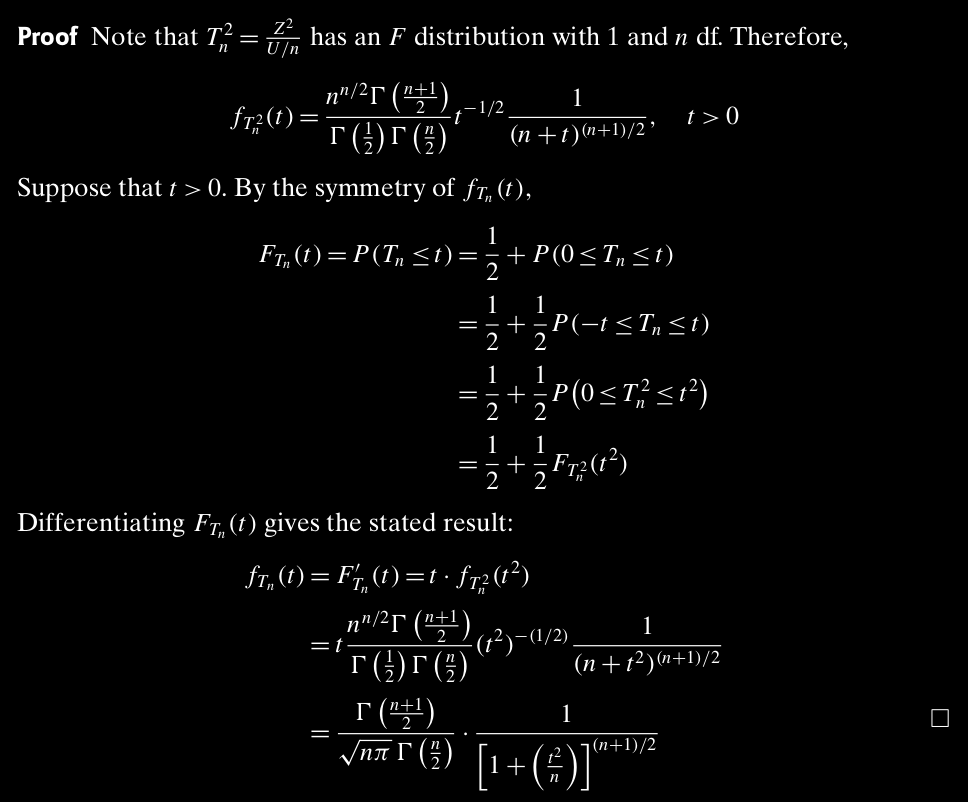
\includegraphics[scale=0.3]{Proof-Theorem-7-3-4-neg.png}
% \end{frame}
% %-------------- end slide -------------------------------%}}}
%-------------- start slide -------------------------------%{{{ 1
\begin{frame}[fragile]
\begin{itemize}
	\item[Proof.] Note that $T_n^2=\frac{Z^2}{U/n}$ follows an $F(1,n)$ distribution. Hence,
		\begin{align*}
			f_{T_n^2} (t) = \frac{n^{\frac{n}{2}}\Gamma(\frac{n+1}{2})}{\Gamma(\frac{1}{2})\Gamma(\frac{n}{2})} t^{-\frac{1}{2}} \frac{1}{(n+t)^{\frac{n+1}{2} }},\quad t> 0.
		\end{align*}
		\item[] Therefore,
		\begin{align*}
			F_{T_n}(t) & = \bbP(T_n\le t)  = \bbP(-\infty< T_n\le 0) + \bbP(0\le T_n\le t).
		\end{align*}
		\item[] The term $\bbP(-\infty< T_n\le 0)$ is a constant which will disappear upon differentiation.
		\item[] Notice that
		\begin{align*}
			\left\{T_n^2 \le t^2 \right\} & = \left\{-t \le T_n \le t\right\} = \left\{-t\le T_n \le 0\right\} \cup \left\{0\le T_n\le t\right\}\\
                                    & = \left\{-t \sqrt{U/n}\le Z \le 0\right\} \cup \left\{0\le Z\le t\sqrt{U/n}\right\}
		\end{align*}
\end{itemize}
\end{frame}
%-------------- end slide -------------------------------%}}}
%-------------- start slide -------------------------------%{{{ 1
\begin{frame}[fragile]
\begin{itemize}
	\item[]  By symmetry of the distribution of $Z$,
		\begin{align*}
			\bbP\left(-t \sqrt{U/n}\le Z \le 0\right)	= \bbP\left(0\le Z\le t\sqrt{U/n}\right)
		\end{align*}
		\item[] Therefore,
		\begin{align*}
			\bbP\left(T_n^2\le t^2\right) & = \bbP\left(-t \sqrt{U/n}\le Z \le 0\right)	+ \bbP\left(0\le Z\le t\sqrt{U/n}\right)\\
			& = 2 \bbP\left(0\le Z\le t\sqrt{U/n}\right)\\
			& = 2 \bbP(0\le T_n \le t).
		\end{align*}
		\item[] Hence,
		\begin{align*}
			F_{T_n}(t) &= const. + \frac{1}{2}\bbP\left(T_n^2\le t^2\right)
		\end{align*}
	\item[] Finally, differentiation gives the density:
	\begin{align*}
		f_{T_n}(t) & = \frac{d}{dt} F_{T_n}(t) = \frac{d}{dt} \frac{1}{2} F_{T_n^2}(t^2) = t\cdot  f_{T_n^2}(t^2) = \cdots .
	\end{align*}
	\myEnd
\end{itemize}
\end{frame}
%-------------- end slide -------------------------------%}}}
%-------------- start slide -------------------------------%{{{ 7.34
\begin{frame}[fragile]
\begin{center}
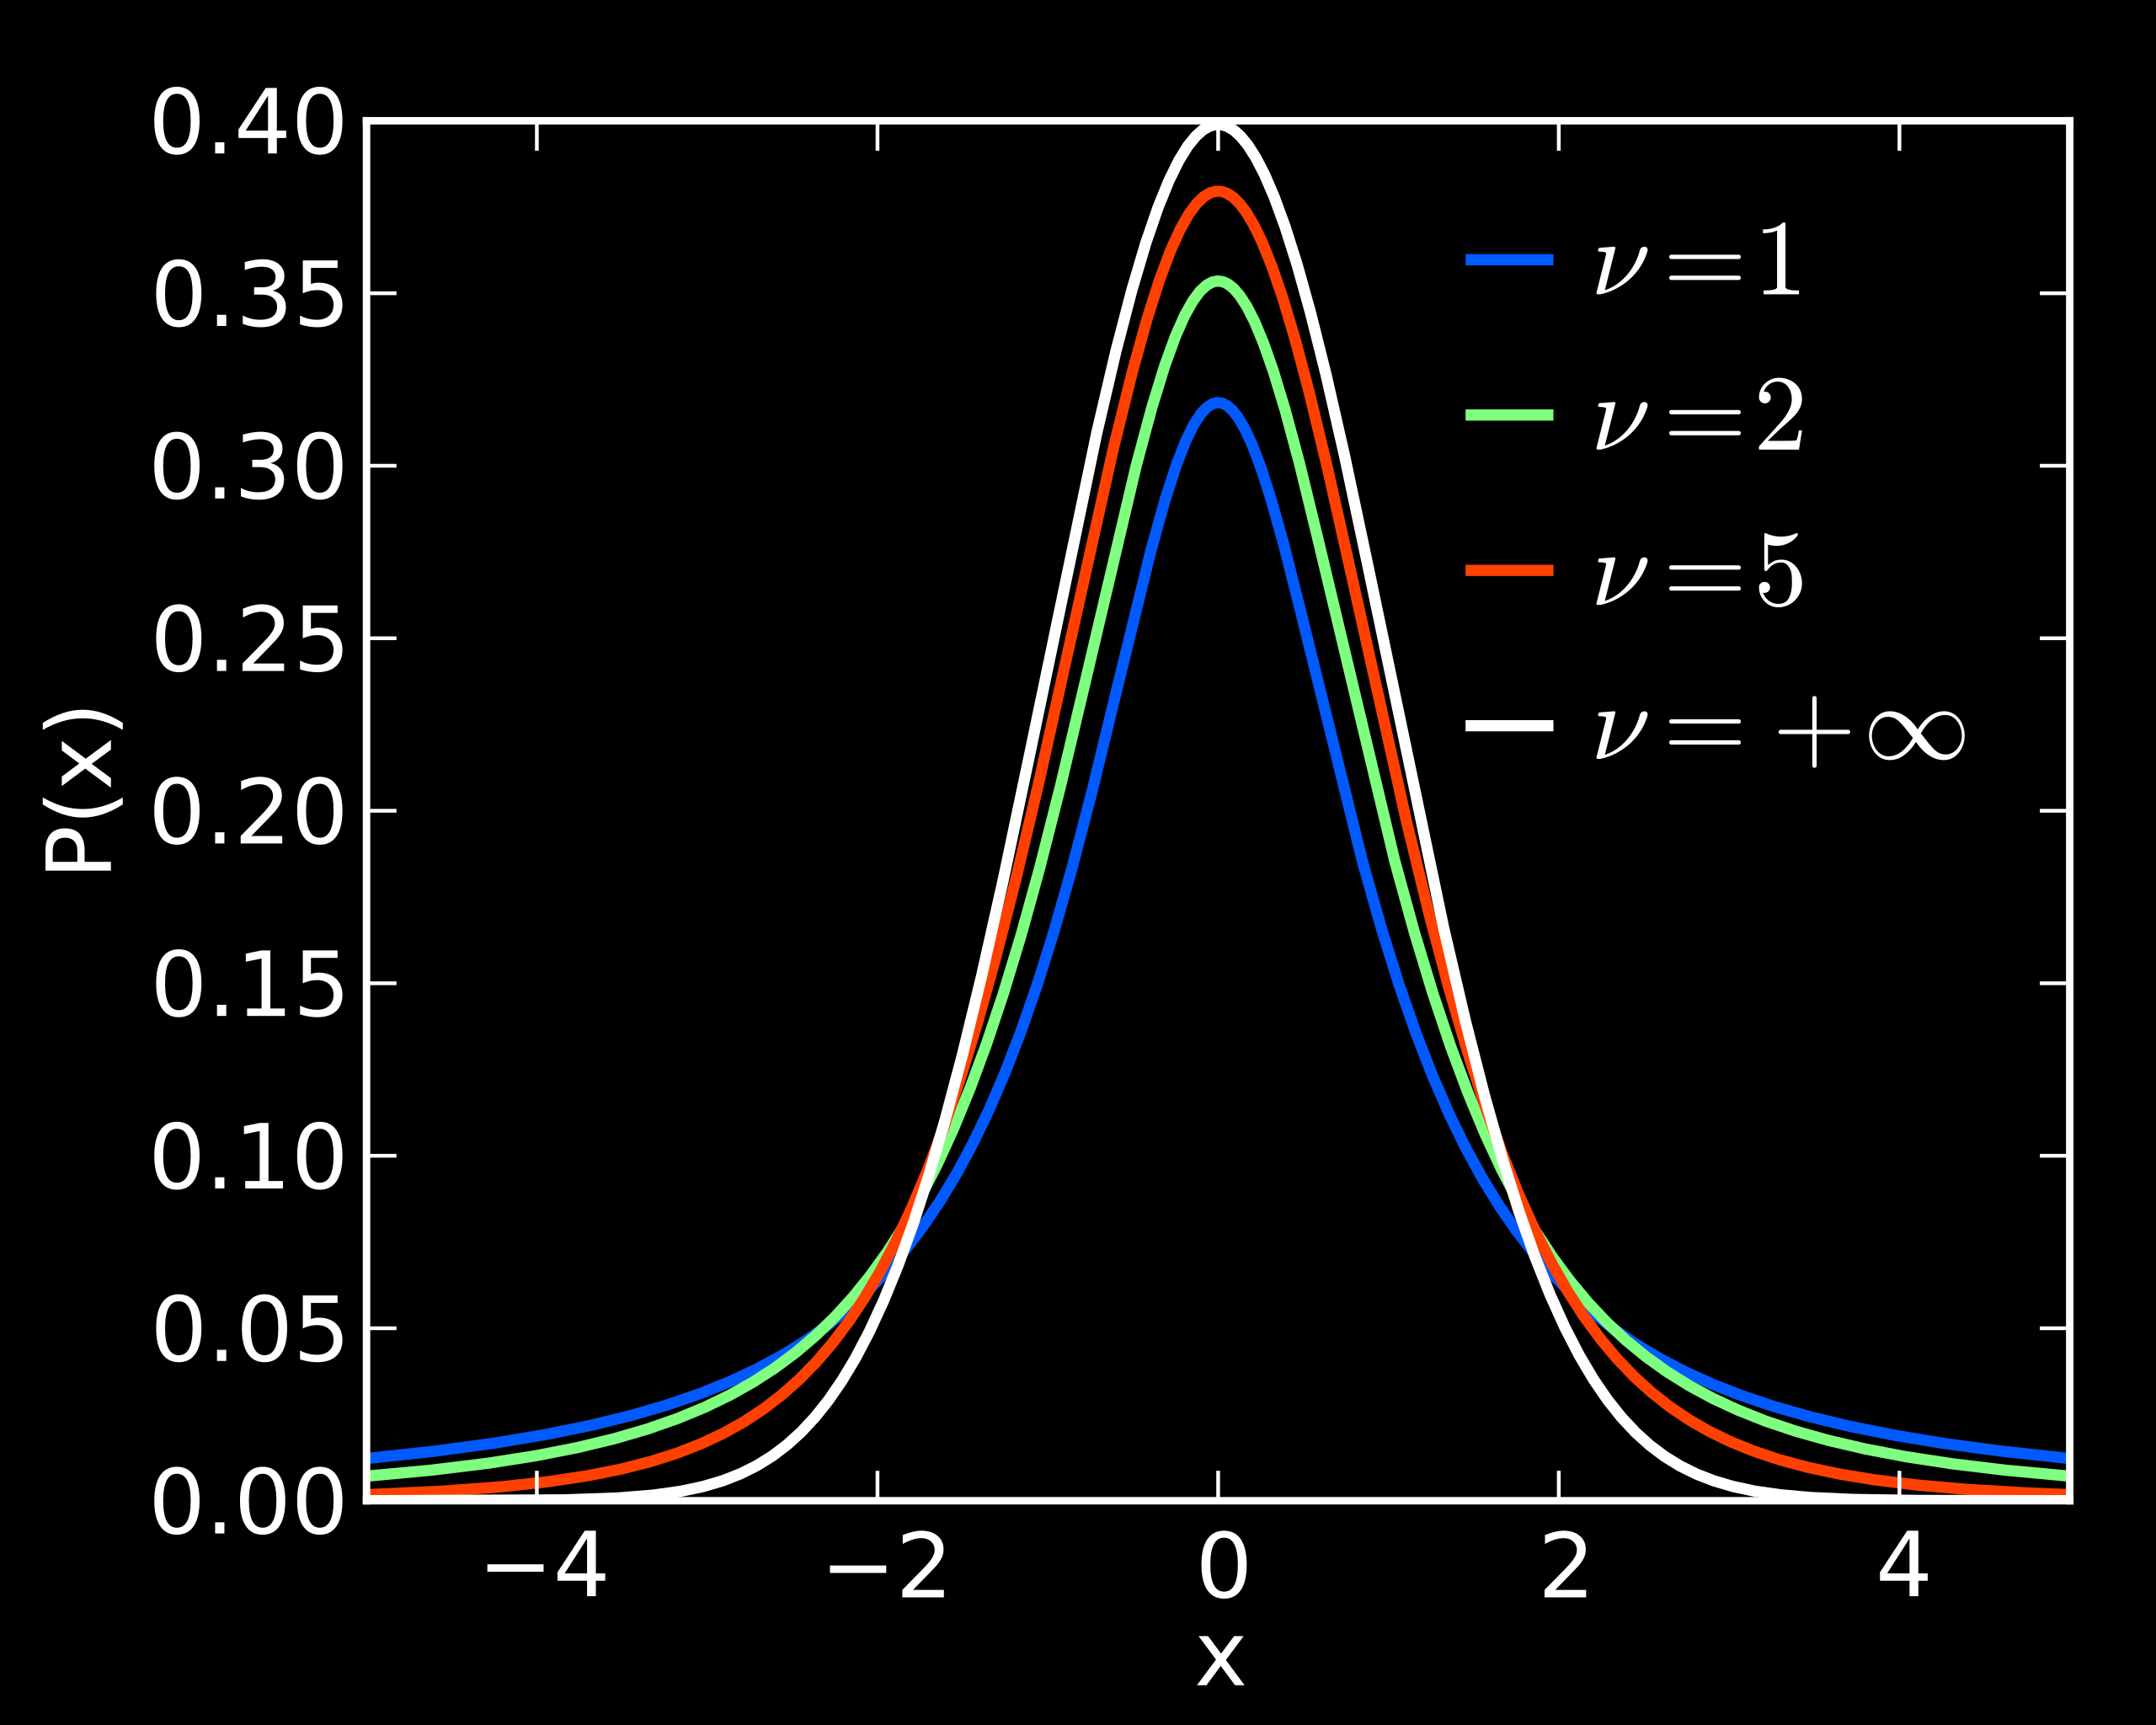
\includegraphics[scale=0.06]{Student_t_pdf-neg.png}\\
\vfill
\begin{minipage}{0.45\textwidth}
\begin{lstlisting}
# Draw Student t-density
x=seq(-5,5,0.01)
pdf= cbind(dt(x, df = 1),
	  			dt(x, df = 2),
	   			dt(x, df = 5),
	   			dt(x, df = 100))
matplot(x,pdf, type = "l")
title("Student's t-distributions")
\end{lstlisting}
\end{minipage}
\end{center}
\end{frame}
%-------------- end slide -------------------------------%}}}
%-------------- start slide -------------------------------%{{{ 7.35
\begin{frame}[fragile]{t Table}
\begin{center}
	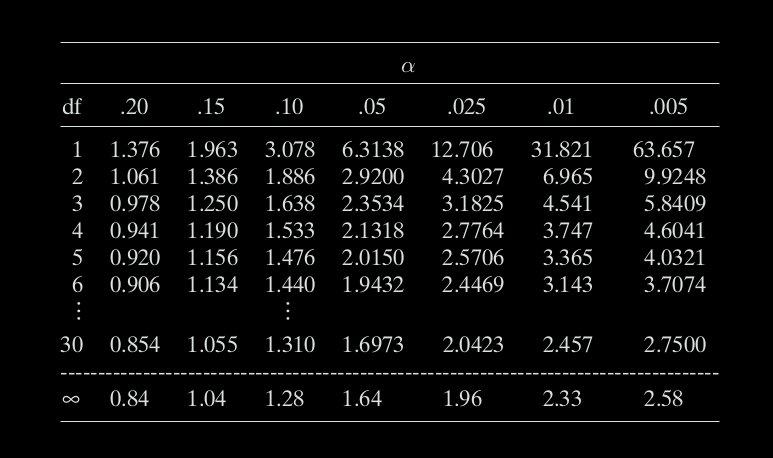
\includegraphics[scale=0.18]{Figure_7-4-1-neg.png}

	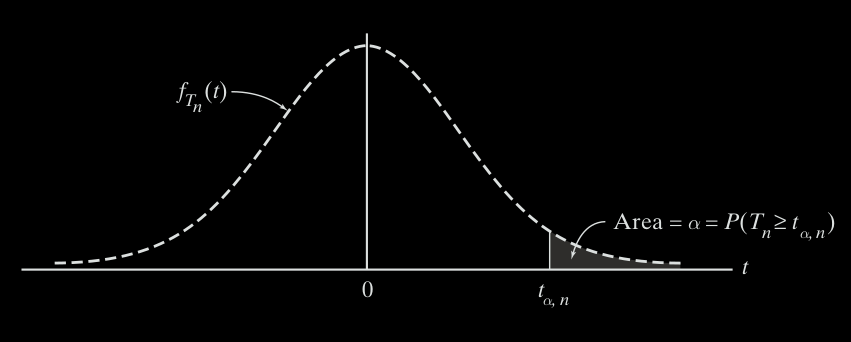
\includegraphics[scale=0.18]{Figure_7-4-2-neg.png}
	\[
		\bbP\left(T_3>4.541 \right) = 0.01 \quad \Longleftrightarrow \quad
		t_{0.01,3} = 4.541
	\]

	\begin{minipage}{0.4\textwidth}
	\begin{lstlisting}
	> 1-pt(4.541, df =3)
	[1] 0.009998238
	\end{lstlisting}
	\end{minipage}
	\qquad
	\begin{minipage}{0.4\textwidth}
	\begin{lstlisting}
	> alpha = 0.01
	> qt(1-alpha, df = 3)
	[1] 4.540703
	\end{lstlisting}
	\end{minipage}
  \vspace{-2em}

	\begin{minipage}{0.4\textwidth}
	\begin{lstlisting}[language=Python]
	> 1 - scipy.stats.t.cdf(4.541, 3)
	[1] 0.00999823806449407
	\end{lstlisting}
	\end{minipage}
	\qquad
	\begin{minipage}{0.4\textwidth}
	\begin{lstlisting}[language=Python]
	> scipy.stats.t.ppf(1-0.01, 3)
	[1] 4.540702858698419
	\end{lstlisting}
	\end{minipage}
\end{center}
\end{frame}
%-------------- end slide -------------------------------%}}}
%-------------- start slide -------------------------------%{{{ 7.36
\begin{frame}
\begin{enumerate}
	\item[Thm \small 7.3.5.] Let $Y_1,\cdots, Y_n$ be a random sample from $N(\mu,\sigma^2)$. Then
		\[
		T_{n-1} = \frac{\overline{Y}-\mu}{S/\sqrt{n}} \quad \sim \quad \text{Student's t of degree $n-1$.}
		\]
	\vfill
	\item[Proof.]
		\[
			\frac{\overline{Y}-\mu}{S/\sqrt{n}}  =  \frac{\displaystyle
				\frac{\overline{Y}-\mu}{\sigma/\sqrt{n}}
			}{
			\displaystyle
			\sqrt{ \frac{(n-1)S^2}{\sigma^2 (n-1)}}
		}
		\]
		\pause\\[1em]
		\[
			\frac{\overline{Y}-\mu}{\sigma/\sqrt{n}}\sim N(0,1)\qquad \perp \qquad
		\frac{(n-1)S^2}{\sigma^2}
		\sim \text{Chi Square$(n-1)$}
		\]
	\\[2em]
	\item[] By Def. 7.3.3 ... \myEnd
\end{enumerate}
\end{frame}
%-------------- end slide -------------------------------%}}}
%-------------- start slide -------------------------------%{{{ 7.37
\begin{frame}
\begin{enumerate}
\item[] As $n\rightarrow \infty$, Students' t distribution will converge to $N(0,1)$: \\
	\begin{center}
		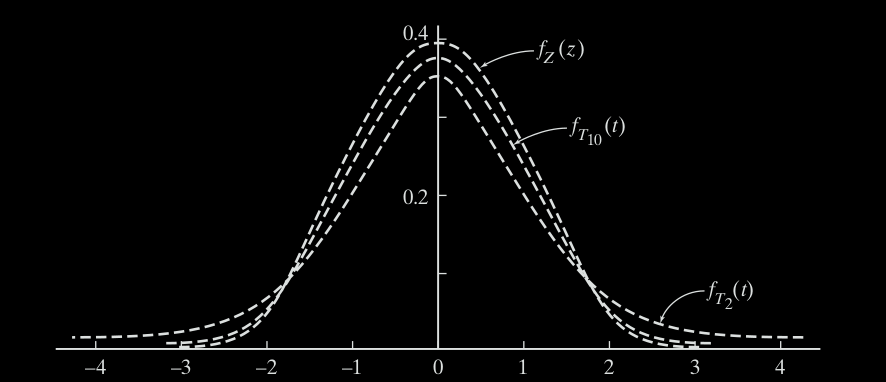
\includegraphics[scale=0.2]{Figure_7-3-2-neg.png}
	\end{center}
\vfill
\item[Thm \small 7.3.6.] $\displaystyle f_{T_n}(x)\rightarrow f_Z(x)= \frac{1}{\sqrt{2\pi}}e^{- \frac{x^2}{2}}\quad $ as $n\rightarrow\infty$, where $Z\sim N(0,1)$.
	\vfill
\item[Proof] By Stirling's formula:
	\[\Gamma(z) =\sqrt{ \frac{2\pi}{z}}\left( \frac{z}{e}\right)^z \left( 1+O(1/z) \right)
		\qquad\text{	as $z\rightarrow\infty$}
	\]
\item[]
	\[
		\Longrightarrow \quad \lim_{n\rightarrow\infty}  \frac{\Gamma\left(  \frac{n+1}{2} \right)}{\sqrt{n \pi}\: \Gamma\left(  \frac{n}{2} \right) } =  \frac{1}{\sqrt{2\pi}}
	\]
	......
	\myEnd
\end{enumerate}
\end{frame}
%-------------- end slide -------------------------------%}}}
